\documentclass[12pt]{exam}
\usepackage[version=4]{mhchem}
\usepackage[usenames,dvipsnames]{color}
\usepackage[T1]{fontenc}
\usepackage{tikz}
\usetikzlibrary{positioning}
\usetikzlibrary{arrows}
\usetikzlibrary{shapes.multipart}
\usepackage[caption=false]{subfig}
\usepackage{tabularx,tikz}
\usepackage{graphicx}
\usepackage{color}
\usepackage{pdfpages}

\pagestyle{headandfoot}
\firstpageheader{Name: \fillin[][4cm]}{Atomic Structure Notes}{Period \fillin[][1cm]}
\firstpagefooter{}{}{}
\runningfooter{Chemistry}{Atomic Structure, Page \thepage\ of \numpages}{\today}

\begin{document}

    
\begin{questions}
        
\section{Atomic Structure}

%!%%%%%%%% ATOMIC NUMBER  %%%%%%%%%%%%%%%
\subsubsection{Atomic Number}


\question The \fillin[atomic number][4cm] is the number of \fillin[protons][3cm] in the nucleus of an atom.

%!%%%%%%%% MASS NUMBER  %%%%%%%%%%%%%%%
\subsubsection{Mass Number}

\question The \fillin[mass number][3cm] is the total number of \fillin[protons][2cm] and \fillin[neutrons][2cm]in the nucleus of an atom.

%*%%%%%% HYDROGEN %%%%%%%

\question In this symbol for Hydrogen: $\ce{^{1}_{}H}$ What does the 1 mean?
\fillin[\# of protons and neutrons][3cm]

%*%%%%%% HELIUM %%%%%%%

\question In this symbol for Helium: $\ce{^{4}_{2}He}$ 

\begin{itemize}
  \item What does the 4 mean? \fillin[\# of protons and neutrons][2cm]
  \item What does the 2 mean? \fillin[\# of neutrons][2cm]
\end{itemize} 

%!%%%%%%%%%%% LITHIUM %%%%%%%%%%%%%%

\question In this symbol for Lithium: $\ce{^{7}_{3}Li}$

\begin{itemize}
  \item How many protons does Lithium have? \fillin[3][2cm]
  \item How many neutrons does Lithium have? \fillin[7 - 3 = 4][2cm]
\end{itemize}

\question based on this symbol: $\ce{^{2}_{}H}$

\begin{itemize}
  \item How many protons does Hydrogen have? \fillin[1][1cm]
  \item How many neutrons? \fillin[1][1cm]
\end{itemize}




%*%%%%%%% BOHR %%%%%%%%%%%%%

\subsection{Bohr Model}

\question   The Bohr Model - Bohr proposed that an atom was a nucleus with electrons "orbiting" in different \fillin[energy levels].

\question Electrons can only have certain energy values known as \fillin[energy levels]


%! ENERGY LEVELS %%%%%%%
\subsubsection{Energy Levels}

\question The electrons closest to the nucleus have the \fillin[lowest] energy, while those further from away have \fillin[higher] energy.

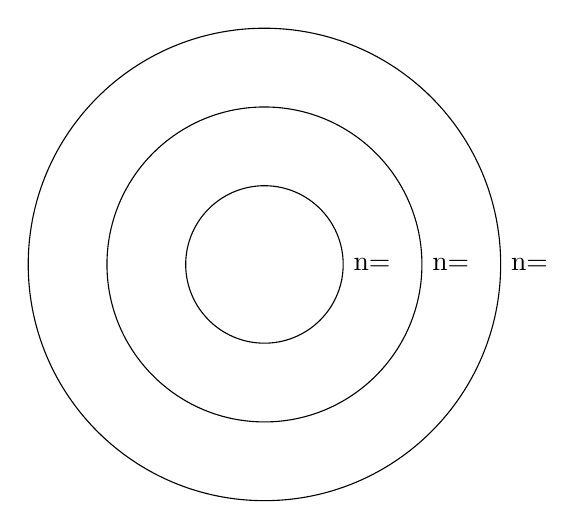
\begin{tikzpicture}
    \foreach \r/\c in {1/n=, 2/n=, 3/n=} 
    {
      \node[circle, draw, minimum size=2*\r cm,label=right:\c] {};
    }
      \end{tikzpicture}


      %! BEGIN PRACTICE
\question draw the electron configuration for \ce{H}
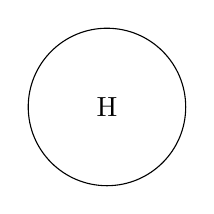
\begin{tikzpicture}
\foreach \r/\c in {1/H} {\node[circle, draw, minimum size=2*\r cm,label=center:\c] {};}
\end{tikzpicture}


\question draw the electron configuration for \ce{He}
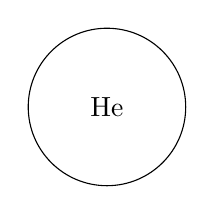
\begin{tikzpicture}
\foreach \r/\c in {1/He} {\node[circle, draw, minimum size=2*\r cm,label=center:\c] {};}
\end{tikzpicture}


\question draw the electron configuration for \ce{Li}
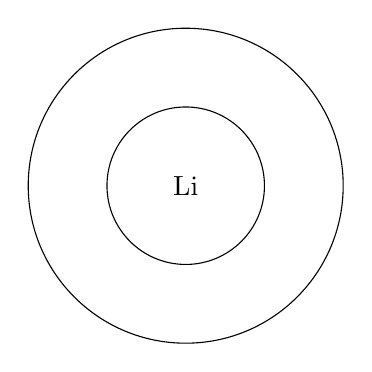
\begin{tikzpicture}
\foreach \r/\c in {1/Li, 2/ } {\node[circle, draw, minimum size=2*\r cm,label=center:\c] {};}
\end{tikzpicture}


\question draw the electron configuration for Boron \ce{B} 
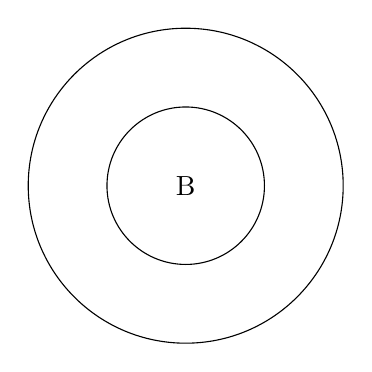
\begin{tikzpicture}
\foreach \r/\c in {1/B, 2/} {\node[circle, draw, minimum size=2*\r cm,label=center:\c] {};}
\end{tikzpicture}


\question draw the electron configuration for Carbon \ce{C} 
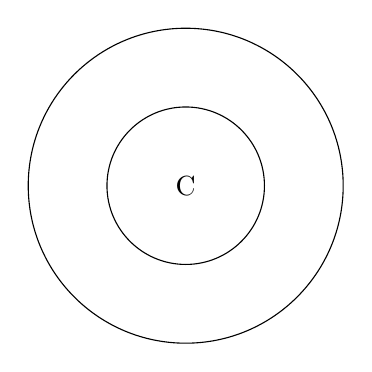
\begin{tikzpicture}
\foreach \r/\c in {1/C, 2/} {\node[circle, draw, minimum size=2*\r cm,label=center:\c] {};}
\end{tikzpicture}

\question draw the electron configuration for Nitrogen \ce{N} 
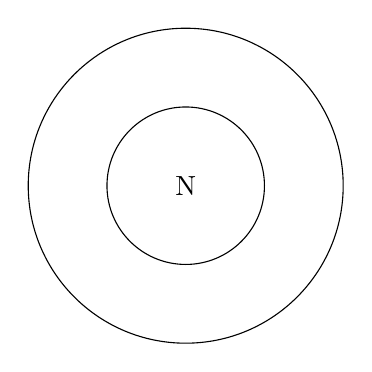
\begin{tikzpicture}
\foreach \r/\c in {1/N, 2/} {\node[circle, draw, minimum size=2*\r cm,label=center:\c] {};}
\end{tikzpicture}


\question draw the electron configuration for Oxygen \ce{O} 
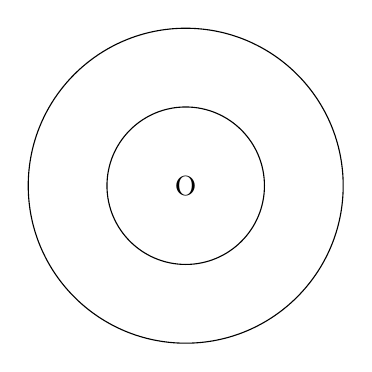
\begin{tikzpicture}
\foreach \r/\c in {1/O, 2/} {\node[circle, draw, minimum size=2*\r cm,label=center:\c] {};}
\end{tikzpicture}

\question draw the electron configuration for Flourine \ce{F} 
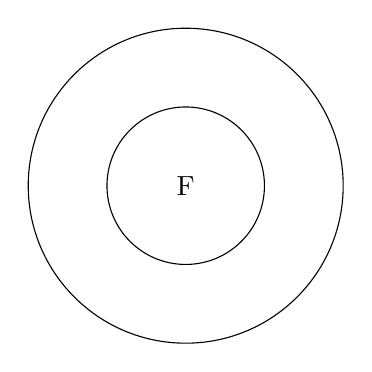
\begin{tikzpicture}
\foreach \r/\c in {1/F, 2/} {\node[circle, draw, minimum size=2*\r cm,label=center:\c] {};}
\end{tikzpicture}


\question draw the electron configuration for Neon \ce{Ne} 
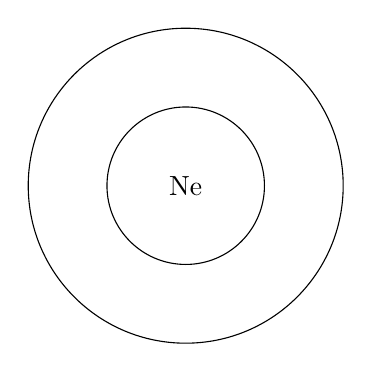
\begin{tikzpicture}
\foreach \r/\c in {1/Ne, 2/} {\node[circle, draw, minimum size=2*\r cm,label=center:\c] {};}
\end{tikzpicture}

%! END PRACTICE

\pagebreak

%%%%%! PERIODIC TABLE %%%%%%%

\section{periodic table}



\question The Periodic Table has \fillin[7][1cm] periods and \fillin[18][1cm] groups.

\question The periods are \fillin[horizontal][3cm] and the groups are \fillin[vertical][3cm]. 

\question You can know the \fillin[electron][3cm] configuration of an element from its \fillin[position][3cm] in the periodic table.

\question The number of electron \fillin[shells][2cm] (or energy levels) is equal to the \fillin[period][2cm] number.

%%%%%%%%%! VALENCE ELECTRONS %%%%%%%%

\question The number of valence electrons is related to the \fillin[group][2cm] number.

\question For atoms in groups \fillin[one][2cm] and \fillin[two][2cm] the number of \fillin[valence][2cm] electrons are equal to the group number.

\question For atoms in groups \fillin[13][2cm] to \fillin[18][2cm] the number of \fillin[valence][2cm] electrons are equal to the group number minus 10.


%! VALENCE ELECTRON PRACTICE 

\subsubsection{Practice}

\question draw the electron configuration for \ce{H}
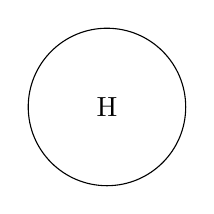
\begin{tikzpicture}
\foreach \r/\c in {1/H} {\node[circle, draw, minimum size=2*\r cm,label=center:\c] {};}
\end{tikzpicture}

How many valence electrons does it have? \fillin[1][1cm]


\question draw the electron configuration for \ce{He}
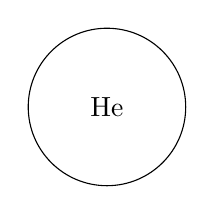
\begin{tikzpicture}
\foreach \r/\c in {1/He} {\node[circle, draw, minimum size=2*\r cm,label=center:\c] {};}
\end{tikzpicture}

How many valence electrons does it have? \fillin[2][1cm]

\question draw the electron configuration for \ce{Li}
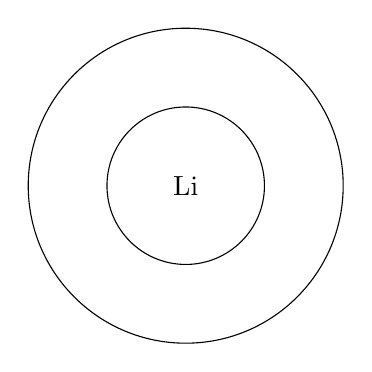
\begin{tikzpicture}
\foreach \r/\c in {1/Li, 2/ } {\node[circle, draw, minimum size=2*\r cm,label=center:\c] {};}
\end{tikzpicture}

How many valence electrons does it have? \fillin[1][1cm]

\question draw the electron configuration for \ce{Be}
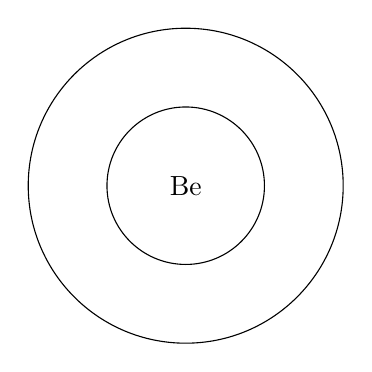
\begin{tikzpicture}
\foreach \r/\c in {1/Be, 2/ } {\node[circle, draw, minimum size=2*\r cm,label=center:\c] {};}
\end{tikzpicture}

How many valence electrons does it have? \fillin[1][1cm]


\question draw the electron configuration for Boron \ce{B} 
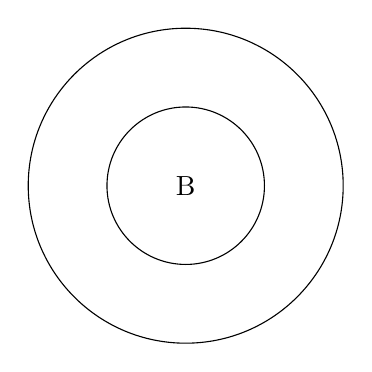
\begin{tikzpicture}
\foreach \r/\c in {1/B, 2/} {\node[circle, draw, minimum size=2*\r cm,label=center:\c] {};}
\end{tikzpicture}

How many valence electrons does it have? \fillin[1][1cm]

\question draw the electron configuration for Carbon \ce{C} 
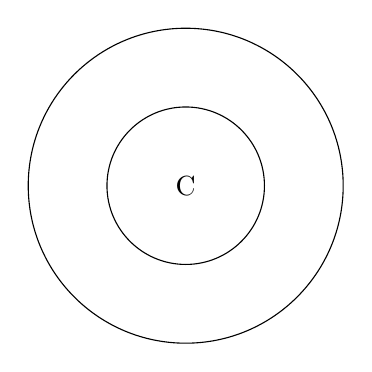
\begin{tikzpicture}
\foreach \r/\c in {1/C, 2/} {\node[circle, draw, minimum size=2*\r cm,label=center:\c] {};}
\end{tikzpicture}

How many valence electrons does it have? \fillin[1][1cm]

\question draw the electron configuration for Nitrogen \ce{N} 
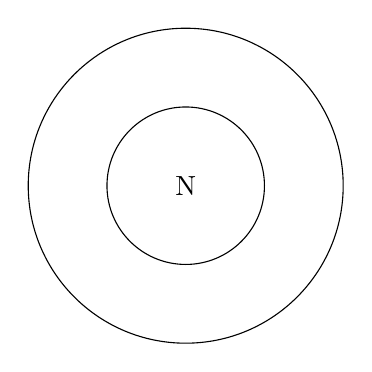
\begin{tikzpicture}
\foreach \r/\c in {1/N, 2/} {\node[circle, draw, minimum size=2*\r cm,label=center:\c] {};}
\end{tikzpicture}

How many valence electrons does it have? \fillin[1][1cm]

\question draw the electron configuration for Oxygen \ce{O} 
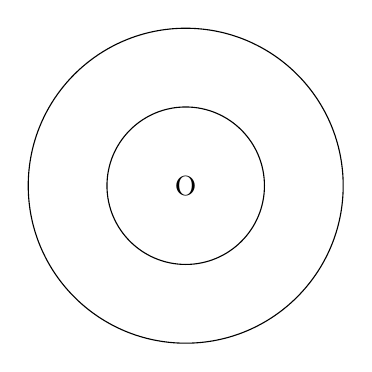
\begin{tikzpicture}
\foreach \r/\c in {1/O, 2/} {\node[circle, draw, minimum size=2*\r cm,label=center:\c] {};}
\end{tikzpicture}

How many valence electrons does it have? \fillin[1][1cm]

\question draw the electron configuration for Flourine \ce{F} 
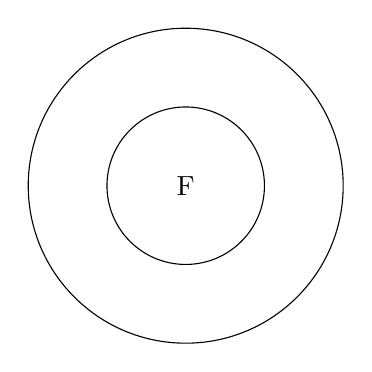
\begin{tikzpicture}
\foreach \r/\c in {1/F, 2/} {\node[circle, draw, minimum size=2*\r cm,label=center:\c] {};}
\end{tikzpicture}

How many valence electrons does it have? \fillin[1][1cm]

\question draw the electron configuration for Neon \ce{Ne} 
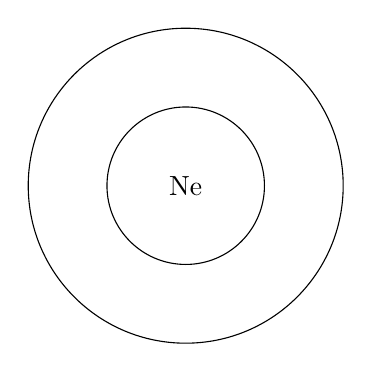
\begin{tikzpicture}
\foreach \r/\c in {1/Ne, 2/} {\node[circle, draw, minimum size=2*\r cm,label=center:\c] {};}
\end{tikzpicture}

How many valence electrons does it have? \fillin[8][1cm]
\end{questions}



\end{document}